\documentclass[a4paper]{article}

%% Language and font encodings
\usepackage[spanish,es-tabla]{babel}
\usepackage[utf8x]{inputenc}
\usepackage{natbib}
\usepackage{booktabs}
\usepackage{tabu}
\usepackage[T1]{fontenc}
\usepackage{subcaption}
\usepackage{float}
\usepackage{amssymb}
\usepackage{multirow}
\usepackage{comment}


%% Sets page size and margins
\usepackage[a4paper,top=3cm,bottom=2cm,left=3cm,right=3cm,marginparwidth=1.75cm]{geometry}

%% Useful packages
\usepackage{amsmath}
\usepackage{graphicx}
%\usepackage{apacite}
\usepackage[colorinlistoftodos]{todonotes}
\usepackage[colorlinks=true, allcolors=blue]{hyperref}

\renewcommand{\labelenumii}{\theenumii}
\renewcommand{\theenumii}{\theenumi.\arabic{enumii}.}

\title{NeoArgos-tools: Un Pipleline de Detección \textit{In-silico} de Neoantígenos de Cáncer para el Desarrollo de Vacunas Personalizadas}

%\title{Desarrollo de una Aplicación Web para la Detección de Neoantígenos en el Marco de Desarrollo %de Vacunas Personalizadas para Tratar el Cáncer }
\author{Vicente Machaca  e Ývan Túpac}
\date{\today}

\begin{document}
	

	
	
	
	
	
	
	
	\maketitle

\part*{Propuesta de la Investigación}

\section{Título}
NeoArgos-tools: Un Pipleline de Detección \textit{In-silico} de Neoantígenos de Cáncer para el Desarrollo de Vacunas Personalizadas.

\section{Lineas de investigación}
Inteligencia Artificial y Áreas transversales.

\section{Áreas de conocimiento OCDE}

	\begin{table}[h]
	\centering
		\setlength{\tabcolsep}{0.5em} % for the horizontal padding
		{\renewcommand{\arraystretch}{1.4}% for the vertical padding
		\begin{tabular}{|p{3cm}|p{10cm}|} \hline
			\textbf{Área} & Ciencias naturales \\ \hline
			\textbf{Sub áreas} &  Informática y Ciencias de la Información \\ \hline
			\textbf{Disciplina} & Bioinformática \\ \hline
			\textbf{URI} &  \href{https://purl.org/pe-repo/ocde/ford\#1.02.03}{https://purl.org/pe-repo/ocde/ford\#1.02.03} \\ \hline
		\end{tabular}}
	\end{table}

	\section{Breve estado de la cuestión}
	
	El cáncer representa el mayor problema de salud mundial \citep{siegel2023cancer}. Además, según el instituto de investigación del cáncer del Reino Unido, se ha registrado más de 18 millones de nuevos casos y 10 millones de muertes en el 2020 \citep{cancerUK2023}. Más alarmante aún, se predice que habrá 28 millones de nuevos casos por año alrededor del 2040, si la incidencia se mantiene estable y el crecimiento de la población y el envejecimiento continúan de acuerdo con las tendencias recientes \citep{cancerUK2023_2}. Esto representa un aumento del 54.9\% con respecto a 2020 y se espera que sea mayor en hombres (aumento del 60.6\%) que en mujeres (aumento del 48.8\%).	A todo esto, se sabe que los métodos tradicionales basados en cirugías, radioterapias y quimioterapias tienen baja efectividad y adversos efectos secundarios \citep{peng2019neoantigen}. En este contexto, surge el desarrollo de la inmunoterapia de cáncer, que tiene como objetivo estimular el sistema inmunológico de un paciente \citep{borden2022cancer}. Existen varios tratamientos como: vacunas personalizadas; terapias de células T adoptivas; e inhibidores de puntos de control inmunológico. De estos, las vacunas basadas en \textbf{neoantígenos} han demostrado un gran potencial, al potenciar las respuestas de las células T y es considerada la de mayor probabilidad de éxito \citep{borden2022cancer}. También, los neantígenos son utilizados en la terapia de bloqueo de puntos de control inmunológico. En este sentido, los neoantígenos son considerados biomarcadores predictivos y objetivos de tratamiento sinérgico en la inmunoterapia del cáncer \citep{fang2022neoantigens}.
	
	
	
	
	El desarrollo de vacunas personalizadas contra el cáncer es un proceso largo y depende de la correcta detección de neoantígenos (ver Figura \ref{fig:vaccines}). Estos neoantígenos son péptidos que solo están presentes en las células cancerosas. De esta forma, el objetivo de un tratamiento basado en vacunas personalizadas, es entrenar a los linfocitos del paciente (células T) para reconocer los neoantígenos y activar el sistema inmunológico \citep{de2020neoantigen, peng2019neoantigen}. El proceso se resume en la Figura \ref{fig:vaccines_b} y consiste en: 
	
	
	
	
	\begin{enumerate}
		\item Obtener muestras de tejido canceroso y saludable, Luego se secuencia ambos tejidos para obtener el ADN y/o ARN. Algunas propuestas incluyen información inmunopeptidoma de \textit{Mass Spectrometry} (MS).
		\item Etapa \textit{in-silico}, aquí realiza alineamiento de secuencias, se desarrolla un \textit{llamado de variantes} para detectar las variantes y/o mutaciones; y se anotan dichas variantes (detección de posibles neoantígenos). Esta etapa cuenta con varias herramientas con buen desempeño.
		\item En esta etapa \textit{in-silico} se priorizan neoantígenos. Esta etapa es crucial y ha tenido bastante investigación los últimos años debido a su complejidad y la baja efectividad de propuestas actuales. Aquí, se toman los neoantígenos candidatos (péptidos) de la etapa anterior y se predice su afinidad con el \textit{Major Histocompatibility Complex} (MHC), este problema se conoce como \textit{pMHC binding}. Luego, se  evalúa la afinidad del pMHC para enlazarse al T-cell Receptor (TCR). Al finalizar esta etapa, se obtienen los neoantígenos.
		\item En esta etapa \textit{in-vitro}, se induce en laboratorio el a las células T del paciente a reconocer los neoantígenos. Aquí, se desarrollan las vacunas. Generalmente, esta etapa es desarrollada por biotecnólogos y biólogos.
		\item Finalmente, el médico oncólogo realiza la evaluación clínica de la vacuna.
	\end{enumerate}
	
	
	
	
	
	
	
	% AGREGAR LOS PIPELINES AGRUPADOS PAOR LA HERRAMITNAS QUE USAN, POR JEMPLO LA MAYORIA DE PIPELINES USAN XXX PARA ALINEAMIENT  Y  XXX PARA, LUEGO LU ...


\begin{figure}[h]
	\centering
	\begin{subfigure}[b]{0.52\textwidth}
		\centering
		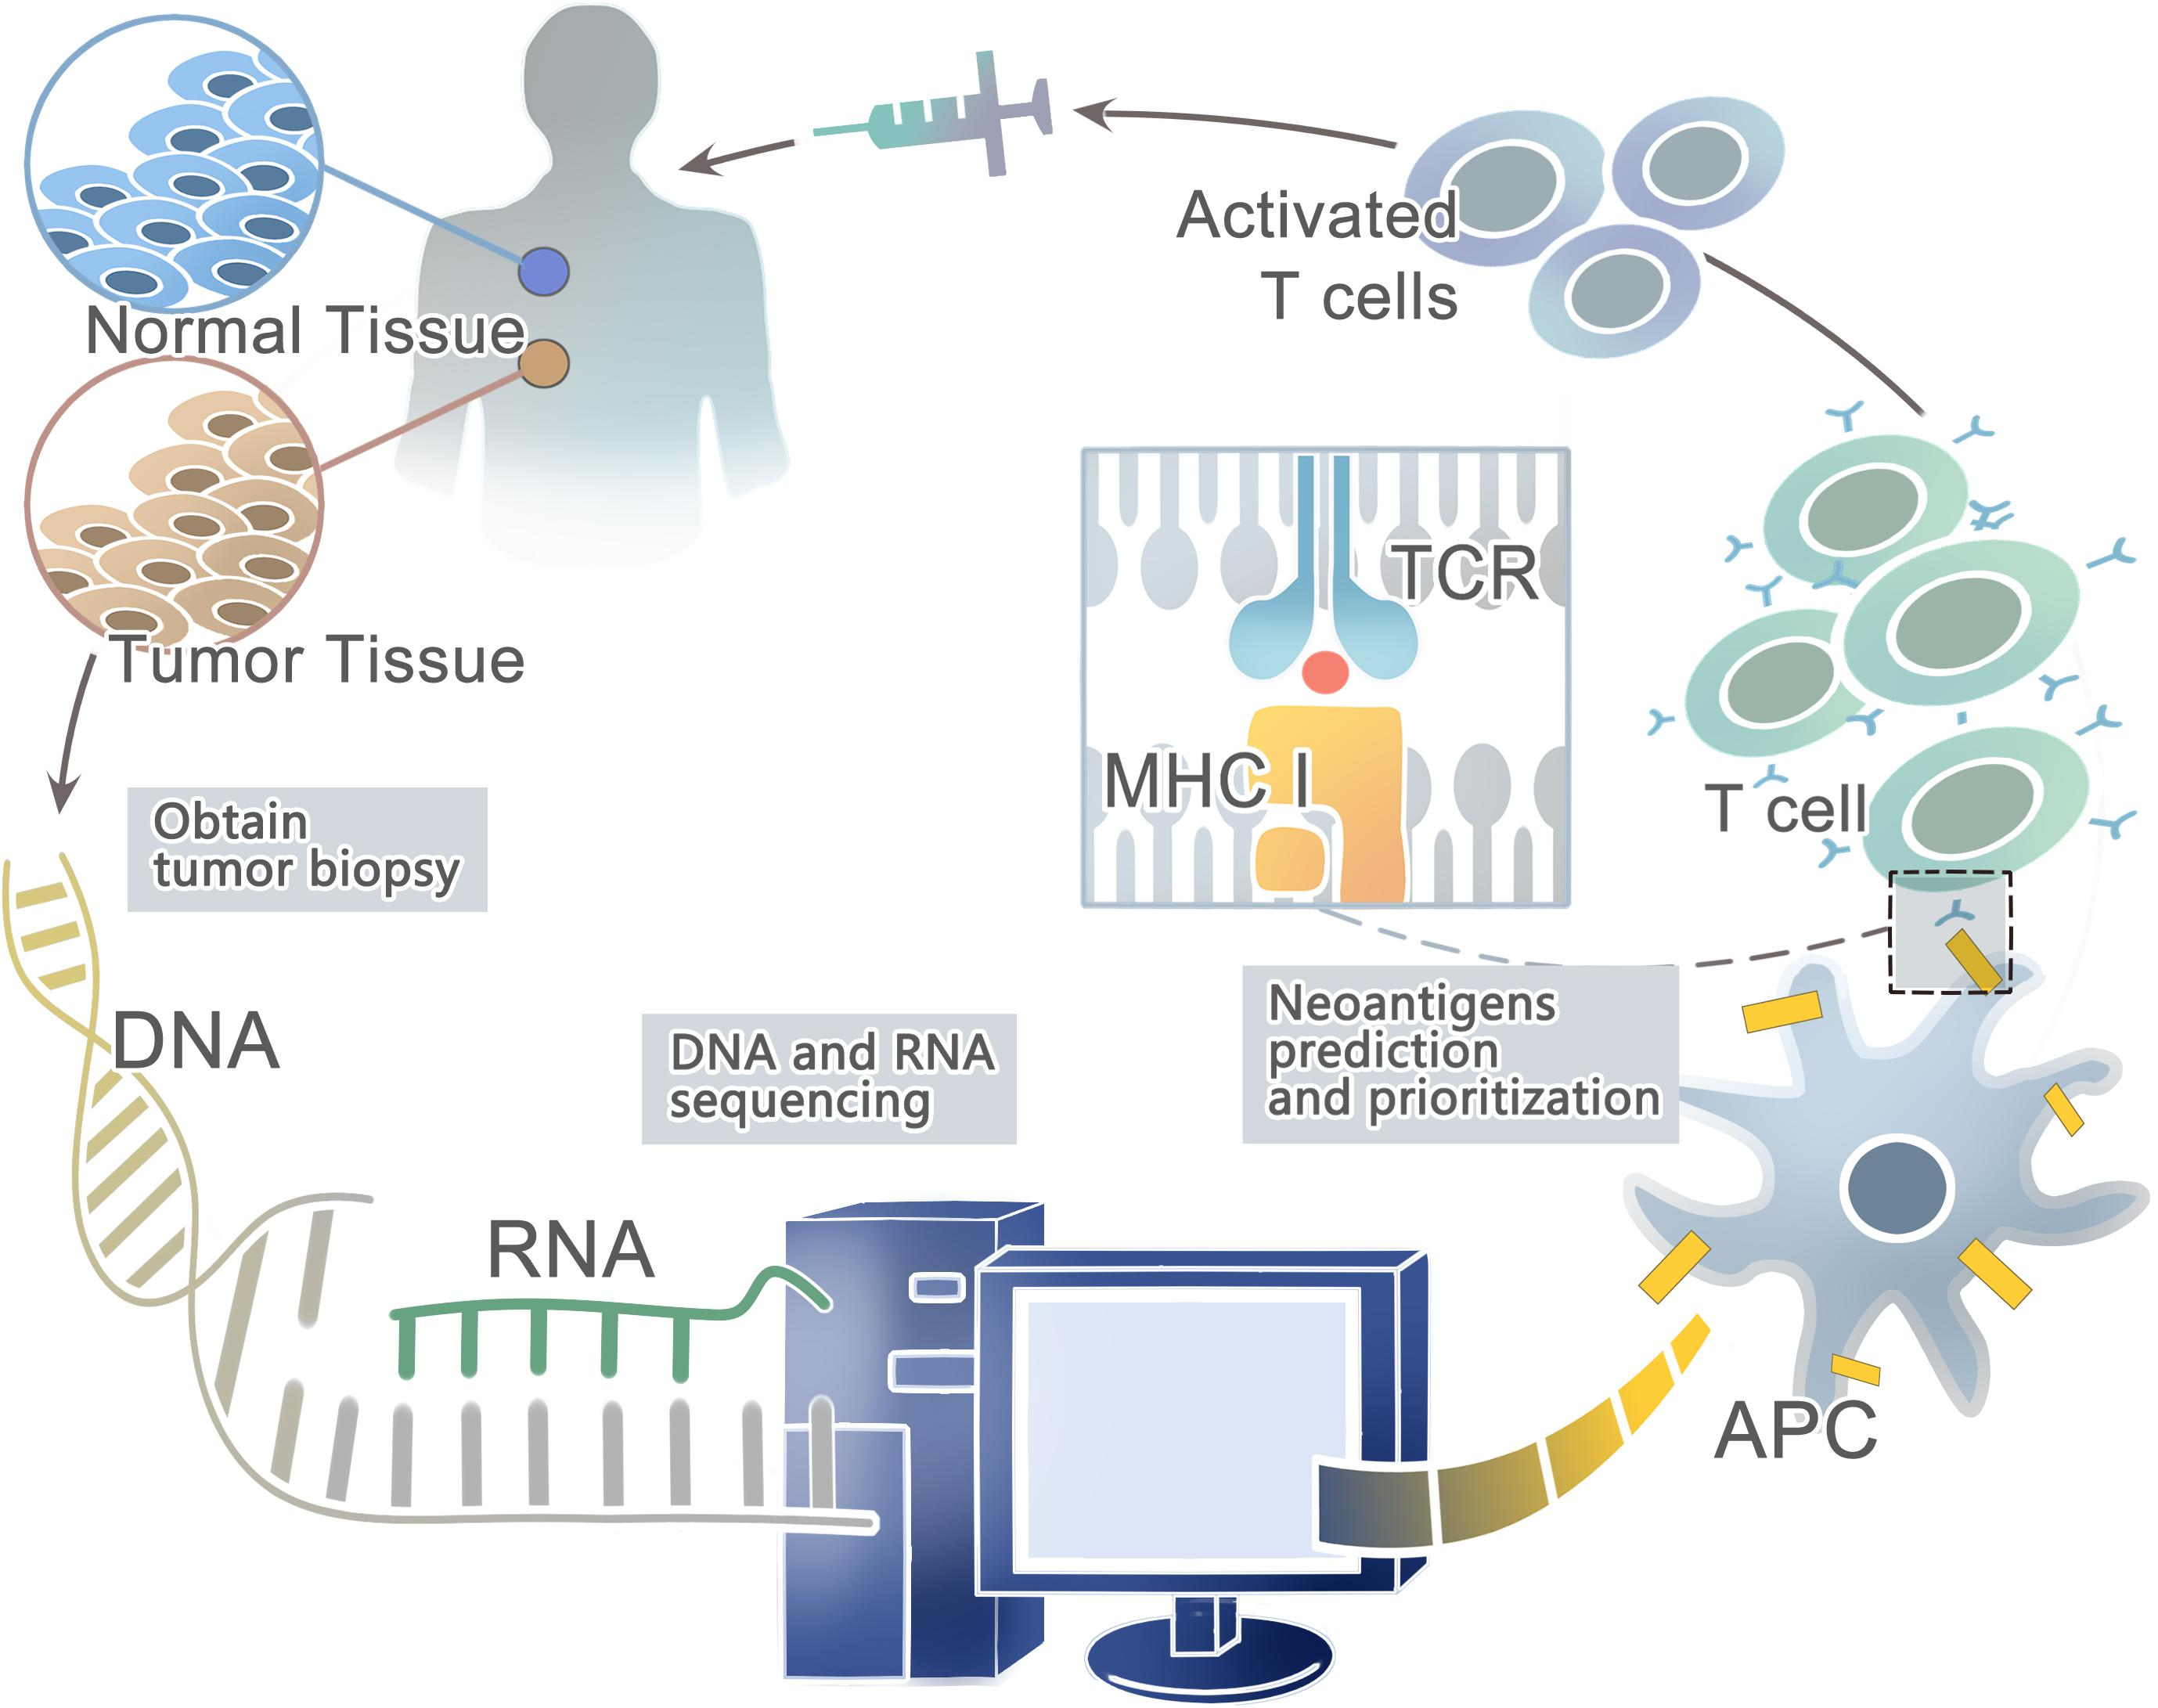
\includegraphics[width=\textwidth]{../img/vaccines/vaccine_pipeline}
		\caption{Proceso de desarrollo de vacunas.}
		\label{fig:vaccines_a}
	\end{subfigure}
	\hfill
	\begin{subfigure}[b]{0.44\textwidth}
		\centering
		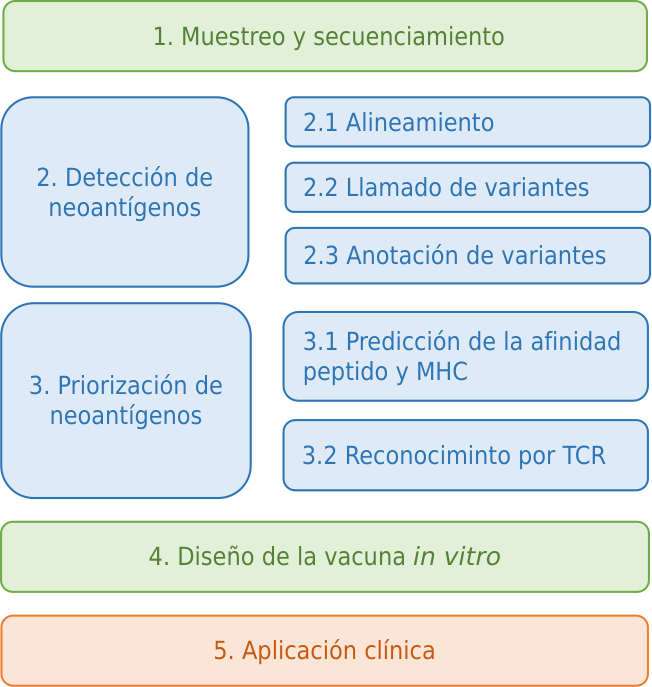
\includegraphics[width=\textwidth]{../img/vaccines/pipeline}
		\caption{\textit{Pipeline} para el desarrollo de vacunas.}
		\label{fig:vaccines_b}
	\end{subfigure}
	
	\caption{Marco de desarrollo para la elaboración de vacunas personalizadas contra el cáncer basadas en neoantígenos. (a) muestra un panorama general de cada etapa. (b) detalla cada fase enfatizando el desarrollo \textit{in-silico}.  Modificado de \cite{han2020progress}.}
	\label{fig:vaccines}
\end{figure}
	
	
La detección \textit{in-silico} de neoantígenos se basa en la segunda y tercera etapa de la Figura \ref{fig:vaccines_b}. En este contexto, debido a la complejidad del proceso y la cantidad de métodos existentes, se han desarrollado software y \textit{pipelines} para facilitar el uso de estas herramientas. En la Tabla \ref{tab:review_pipelines}, presentamos los \textit{pipelines} publicados a partir del 2018. Estos \textit{pipelines} utilizan diferentes tipos de información como entrada, así PGV Pipeline \citep{rubinsteyn2018computational} y PEPPRMINT \citep{zhou2023prioritizing} utilizan DNA-seq; sin embargo, otras herramientas como PGNneo \citep{tan2023pgnneo}, NAP-CNB \citep{wert2021predicting}, NaoANT-HILL \citep{coelho2020neoant}, ProGeo-neo \citep{li2020progeo}, ScanNeo \citep{wang2019scanneo} y Neopepse \citep{kim2018neopepsee} utilizan RNA-seq porque estas secuencias encapsulan mejor la información de mutaciones y \textit{non-coding regions} de ADN \citep{tan2023pgnneo}. 

Con el objetivo de reducir la complejidad de los \textit{pipelines}, otras propuestas han optado por utilizar Variant Calling Format (VCF), como entrada. Estos archivos, contienen información de las mutaciones y son obtenidas a partir de métodos de alineamiento y llamado de mutaciones (etapas 2.1 y 2.2 de la Figura \ref{fig:vaccines_b}). De esta forma, herramientas como Valid-Neo \citep{terai2022valid}, HLA3D \citep{li2022hla3d}, Neoepiscope \citep{wood2020neoepiscope} , pVACtools \citep{hundal2020pvactools} y NeoPredPipe \citep{schenck2019neopredpipe}, reducen la cantidad de herramientas utilizadas en la deteccion de neoantígenos; sin embargo, los resultados obtenidos, pueden ser inferiores comparado con herramientas que usan DNA-seq y RNA-seq.

Adicionalmente, para una correcta detección de neoantígenos, es necesario contar con la secuenciación de proteínas Major Histocompatibility Complex (MHC) o Human Leukocyte Antigens (HLA). Es necesario contar con estas proteínas porque, son utilizadas para predecir la unión entre posibles neoantígenos al MHC (pMHC: etapa 3.1 de la Figura \ref{fig:vaccines_b}). Estas proteínas son codificadas por genes altamente polimórficos, esto proporciona una variación sustancial en la unión de péptidos (neoantígenos), influyendo de esta manera en el conjunto de péptidos presentados a las células T. \citep{abualrous2021major}. En este contexto,  los \textit{pipelines} Valid-NEO \citep{terai2022valid}  y NeoPredPipe \citep{schenck2019neopredpipe} y Neopepsee \citep{kim2018neopepsee} solicitan como entrada estas proteínas (HLA); mientras que las otras predicen esta información a partir de DNA-seq. Desde un punto de vista de usabilidad, obtener los tipos de HLA, implica un esfuerzo inncesario para el usuario.

En resumen, el desarrollo de \textit{pipelines} para la detección de neoantígenos es un campo de investigación significativo y de gran envergadura. Además, se está viendo favorecido por el crecimiento exponencial de la información genómica y los avances recientes en inteligencia artificial. Esto ha generado una fuerte demanda de investigaciones interdisciplinarias que integran las disciplinas de la ciencia de la computación y la biología molecular.



% falta mencioan porque usan MS


	
\begin{table}[h]
	\caption{Lista de \textit{pipelines} desarrollados desde el 2018 hasta la actualidad para la detección de neoantígenos.}
	\label{tab:review_pipelines}
	\setlength{\tabcolsep}{0.5em} % for the horizontal padding
	{\renewcommand{\arraystretch}{1.5}% for the vertical padding
		
	
			\begin{tabular}{lp{0.6cm}p{3cm}p{4.5cm}p{2.7cm}}
	\textbf{Nombre} & \textbf{Año}  & \textbf{Ref.}                                 & \textbf{Entrada}                                         & \textbf{Salida}                                     \\ \hline
	
	PEPPRMINT         & 2023 &\cite{zhou2023prioritizing}         & DNA-seq                                                  & Neoantígenos                                        \\

	PGNneo & 2023	& \cite{tan2023pgnneo}	& VCF, RNA-seq y MS data	& Neoantígenos \\
	
	Valid-NEO       & 2022 &\cite{terai2022valid}             & VCF y HLA          & Neoantígenos  \\
	
	HLA3D & 2022	& \cite{li2022hla3d}	& VCF, HLA, SMG y HBV	& Neoantígenos \\
	
	
	
	NAP-CNB         & 2021 &\cite{wert2021predicting}         & RNA-seq                                                  & Neoantígenos                                       \\
	
	NeoANT-HILL     & 2020 &\cite{coelho2020neoant}           & RNA-seq y VCF                        & Neoantígenos y gene expression  \\
	
	Neoepiscope     & 2020 &\cite{wood2020neoepiscope}        & VCF y BAM                   & Neoantígenos y mutaciones                          \\
	
	ProGeo-neo      & 2020 &\cite{li2020progeo}               & RNA-seq y VCF                        & Neoantígenos                                       \\
	
	pVACtools       & 2020 &\cite{hundal2020pvactools}        & VCF                                         & Neoantígenos                                       \\
	
	NeoPredPipe     & 2019 &\cite{schenck2019neopredpipe}     & VCF y HLA                            & Neoantígenos y variant annotation              \\
	
	ScanNeo         & 2019 &\cite{wang2019scanneo}            & RNA-seq                                                  & Neoantígenos                                       \\
	
		
	Neopepsee       & 2018 &\cite{kim2018neopepsee}           & RNA-seq, VCF, HLA  & Neoantígenos y gene expression    \\ 
	
	PGV Pipeline    & 2018 &\cite{rubinsteyn2018computational}& DNA-seq                                                  & Neoantígenos                                       \\
	
	
	
	
	
\end{tabular}
	
	}
\end{table}




\section{Planteamiento del problema}

A pesar de varios esfuerzos en el desarrollo de \textit{pipelines} y algoritmos, menos del 5\% de neoantígenos detectados activan el sistema immune \citep{de2020neoantigen, mill2022neoms, bulik2019deep, bassani2015mass, yadav2014predicting}. Según los autores de los \textit{pipelines} las razones pueden ser: 

\begin{enumerate}
	\item La no inclución en conjunto de varias fuentes de información como DNA-seq, RNS-seq, y datos de \textit{Mass Spectrometry} (MS)  \citep{kim2018neopepsee}.
	\item  Uso herramientas de bajo desempeño para la predicción del enlace péptido-MHC (pMHC) (etapa 3.1  de la Figura \ref{fig:vaccines_b}). La mayoria de aplicaciones, se basa en el uso de MHCFlurry \citep{o2020mhcflurry} y NetMHCpan4.1 \citep{reynisson2020netmhcpan}. En la actualidad, se cuenta con herramientas de mejor desempeño basado en transformers \citep{arceda2023neoantigen}.
	\item Para la etapa 3.2 de la Figura \ref{fig:vaccines_b}, los autores no consideran  la predicción del pMHC al TCR, la mayoria comenta incluir esta tarea en trabajos futuros  \citep{rubinsteyn2018computational}.
	\item Finalmente y quizas la mas importante es no utilizar información de eventos de \textit{alternative splicing}, variaciones estructurales en el ADN y las mutaciones de fusión de genes, está información esta fuertemente relacionada con varios tipos de cancer \citep{wood2020neoepiscope}.
\end{enumerate}

	
\section{Objetivos de la investigación}
	
	\subsection{Objetivo general}
	
	Desarrollar el \textit{pipeline} NeoArgos-tools de detección \textit{in-silico} de neoantígenos de cáncer para el desarrollo de vacunas personalizadas.
	
	\subsection{Objetivos específicos}
	\begin{enumerate}
		\item Analizar que fuentes de información o datos de entrada recibirá el \textit{pipeline}. Se evaluará DNA-seq, RNA-seq, VCF y datos de MS.
		
		\item Analizar que herramientas se van a utilizar para la primera etapa del \textit{pipeline}, referente al alineamiento de secuencias, llamado de variantes y  anotación de variantes (predicción de posibles neoantígenos). 
		
		\item Analizar el uso de información de variaciones estructurales del ADN y mutaciones de fusión de genes. Se evaluará el desempeño de \textit{Arriba} \citep{uhrig2021accurate} y FusionQ \citep{liu2013fusionq}.
		 
		\item Implementar un modelo basado en transformers para la predicción del enlace de los neoantígenos al MHC (pMHC). Ya se cuenta con resultados previos de una propuesta que es superior a otras del estado del arte \citep{arceda2023neoantigen}.
		
		\item Integrar las herramientas evaluadas y seleccionadas en un contenedor con Docker.
		\item Comparar el desempeño del \textit{pipeline} con otras herramientas del estado del arte.

		

		
	\end{enumerate}

	
\section{Importancia de la investigación}

El cáncer es el mayor problema de salud mundial; sin embargo, los métodos tradicionales basados en cirugías, radioterapias y quimioterapias tienen baja efectividad \citep{peng2019neoantigen}. En este contexto, los neoantígenos son factores clave en el desarrollo de vacunas contra el Cáncer  \citep{borden2022cancer,chen2021challenges,gopanenko2020main}. Si se logra desarrollar un método con un buen desempeño, la inmunoterapia del cáncer basada en el desarrollo de vacunas personalizadas, podría utilizarse como alternativa a otros métodos como radioterapias y quimioterapias. \\

En el área de ciencia de la computación existen dos contribuciones importantes. Primero en el campo inteligencia artificial y específicamente en el tópico de \textit{deep learning}, el desarrollo de un método basado en \textit{transformers} para la predicción del enlace pMHC, representa una contribución importante  y demuestra que este tipo de modelos no solo pueden utilizarse en campos del procesamiento natural del lenguaje (como lo hace chatGPT) sino también en otros ámbitos como la Immunoinformática. Luego, el desarrollo propio del \textit{pipeline}, representa un reto en la ingeniería de software, resolviendo problemas de integración, alto costo computacional, heterogeneidad y modularidad. De esta forma, se tiene como objetivo desarrollar un \textit{pipeline} con mejor desempeño a otros del estado del arte al incorporar información de Mass Spectrometry (MS) y fusión de genes.\\ 

Finalmente, tener una aplicación de detección de neoantígenos desarrollada por la Universidad La Salle y la Universidad Católica San Pablo, realza el nombre de ambas universidades y demuestra que gracias al trabajo en conjunto se puede desarrollar aplicaciones de gran envergadura aplicadas a campos multidisciplinarios y nos alinea a grandes instituciones como el European Molecular Biology Laboratory (EMBL) y el National Institutes of Health (NIH).




\section{Diseño y secuencia lógica de la investigación} 

Hemos dividido la propuesta en dos módulos NeoArgosMut y NeoArgosAntigen. NeoArgosMut, se enfoca en el llamado y anotación de variantes, como salida se obtiene neoantígenos candidatos. Luego, NeoArgosAntigen, prioriza estos antígenos, al predecir su afinidad al MHC (pMHC) y luego la afinidad del pMHC al TCR (pMHC-TCR). En la Figura \ref{fig:pipeline}, mostramos estos módulos. Adicionalmente, ya contamos con resultados previos para NeoArgosAntigen de dos trabajos anteriores: hemos desarrollamos una revisión sistemática de la literatura \citep{machaca2023deep} y también hemos experimentado el \textit{transformers} y \textit{transfer learning} para la predicción del enlace pMHC \citep{arceda2023neoantigen}. Actualmente, contamos con modelos con un desempeño superior a otros del estado del arte.


\begin{figure}[h]	
		\centering
		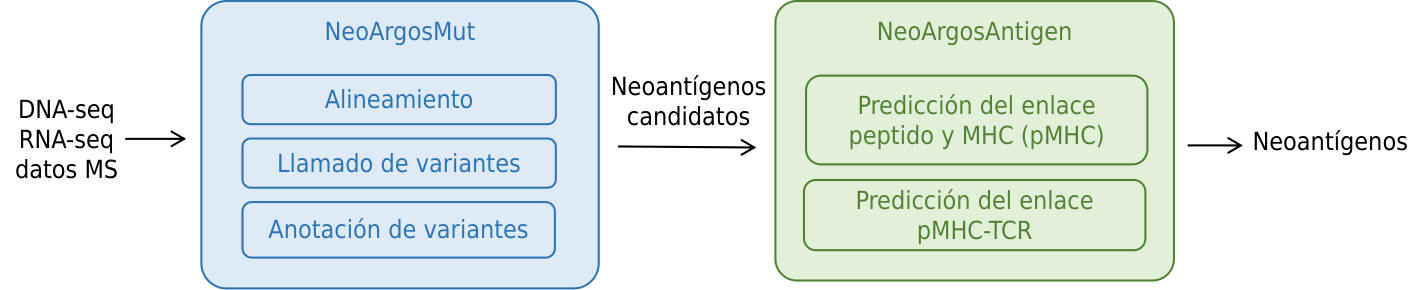
\includegraphics[width=\textwidth]{../img/pipeline/proposal_pipeline}	
	\caption{Representación de NeoArgosMut y NeoArgosAntigen para la detección de neoantígenos}
	\label{fig:pipeline}
\end{figure}


\subsection{NeoArgosMut}

NeoArgosMut, se encarga de recibir como entrada datos de DNA-seq, RNA-seq y Mass Spectrometry (MS). Luego se plantea alinear dichas secuencias con uso de las herramientas como BWA-MEM \citep{li2013aligning}, Bowtie2 \citep{langmead2012fast}. Adicionalmente, se usará STAR \citep{dobin2013star} porque alinea mejor muestras tumorales \citep{rubinsteyn2018computational}. Como salida a esta etapa, se optiene archivos de alineamiento BAM.\\

Para el llamado de variantes se utilizará MuTect \citep{cibulskis2013sensitive} y Strelka \citep{saunders2012strelka}. Luego, se utilizará la unión de la información de ambos métodos tal como lo hizo \cite{zhou2023prioritizing} y \cite{rubinsteyn2018computational}. Como salida, se obtienen archivos VCF. Adicionalmente a otros \textit{pipelines}, utilizaremos información sobre la fusión de genes que se obtendrán de las herramientas \textit{Arriba} \citep{uhrig2021accurate} y FusionQ \citep{liu2013fusionq}. Esta forma parte de la contribución de este trabajo, porque se sabe que la mayoría de \textit{pipelines} tienen un bajo desempeño debido ausencia de información en su procesos de variantes estructurales y fusión de genes \citep{wood2020neoepiscope}. Finalmente, también se va a utilizar MaxQuant \citep{cox2008maxquant} para identificar las mutaciones a nivel de péptidos con ayuda de información de Mass Spectrometry (MS), esto también forma parte de la contribución del trabajo al incluir fuentes adicionales de información como MS.\\



Luego corresponde a la anotación de variantes, en esta etapa se toman los archivos en formato VCF y se obtienen los péptidos generados a partir de estas variaciones o mutaciones. Estos péptidos representan los posibles neoantígenos. Para está tarea se va a utilizar Isovar y ANNOVAR \citep{wang2010annovar}. \\

Finalmente, para obtener el tipo de HLA del paciente se va a utilizar la herramienta OptiType \citep{szolek2014optitype}. Otros \textit{pipelines} optan por solicitar al usuario la información del tipo de HLA; sin embargo, obtener el HLA a partir de las mismas secuencias de ADN, mejora considerablemente el desempeño general del pipeline y la accesibilidad del usuario.




\subsection{NeoArgosAntigen}

NeoArgosAntigen, prioriza los neoantígenos detectados previamente por NeoArgosMut. Esta priroización la realiza en base a la predicción del enlace de los neoantígenos al MHC y posteriormete al TCR. El módulo se divide en dos partes: la predicción del enlace pMHC y la afinidad del pMHC al TCR. Ambas toman como entrada dos secuencias de proteínas, luego se necesita predecir su afinidad (regresión) o el enlace (clasificación). En resumen, las proteínas se pueden representar como $p = \{ A, ... , Q \}$ y $q = \{ A, N, ... ,Q, E, G \}$. Luego, tenemos que  predecir la probabilidad del enlace o afinidad entre $p$ y $q$. \\


Para el problema de predicción del enlace pMHC se va a utilizar modelos BERT pre-entrenados y se realizará \textit{fine-tuning} agregando un bloque de capas BiLSTM. Luego se volverá a entrenar estos modelos con una base de datos compuesta por muestras de \cite{zhang2022hlab} y \cite{gfeller2023improved}. Se propone la arquitectura de la Figura \ref{fig:proposal}. Como se puede ver, la entrada son dos secuencias de proteínas: el péptido y el MHC. Luego, el modelo basado en transformers está compuesto por un modelo pre-entrenado y un bloque de capas BiLSTM, esta propuesta se basó en el trabajo de \cite{zhang2022hlab}. En esta etapa también. se va a evaluar el desempeño de varios modelos BERT pre-entrenados como: TAPE \citep{rao2019evaluating}, ProtBERT-BFD \citep{elnaggar2021prottrans} y ESM2 \citep{lin2023evolutionary} cada una con 92 millones, 420 millones, 650 millones parámetros respectivamente. Adicionalmente, TAPE fue entrenado con 30 millones de proteínas, ProtBERT-BFD con 2122 millones de proteínas y 60 millones de proteínas para ESM-2. En base a trabajos anteriores propios, sabemos que el uso de TAPE y el modelo más pequeño de ESM2 tienen buenos resultados \citep{arceda2023neoantigen}.\\




\begin{figure}[H]
	\centering
	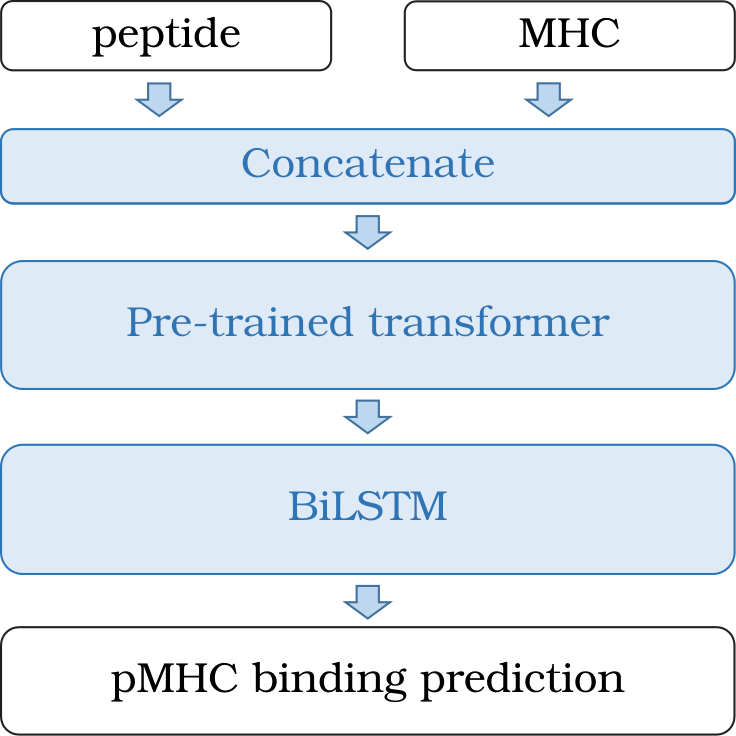
\includegraphics[width=0.35\textwidth]{../img/pipeline/proposal_pmhc}
	\caption{Propuesta: Utilizamos el modelo de transformer ESM2 seguido de BiLSTM para predecir el enlace pMHC.}
	\label{fig:proposal}
\end{figure}

La misma arquitectura de la Figura \ref{fig:proposal}, se utilizará para la predicción del enlace pMHC y TCR (pMHC-TCR) según recomendaciones de \cite{li2020progeo}  y \cite{myronov2023bertrand}. Sin embargo, se va reentrenar el modelo para adaptarse a este nuevo problema, se utilizarán muestras de \cite{li2020progeo} y la base de datos de VDJdb \citep{shugay2018vdjdb}.






	
	\bibliographystyle{apalike}
	\bibliography{../bibliography}

\clearpage


%%%%%%%%%%%%%%%%%%%%%%%%%%%%%%%%%%%%%%%%%%%%%%%%%%%%%%%%%%%%%%%%%%%%%%
%%%%%%%%%%%%%%%%%%%%%%%%%%%%%%%%%%%%%%%%%%%%%%%%%%%%%%%%%%%%%%%%%%%%%%
%%%%%%%%%%%%%%%%%%%%%%%%%%%%%%%%%%%%%%%%%%%%%%%%%%%%%%%%%%%%%%%%%%%%%%
%%%%%%%%%%%%%%%%%%%%%%%%%%%%%%%%%%%%%%%%%%%%%%%%%%%%%%%%%%%%%%%%%%%%%%
\part*{Gestión del Proyecto}

\setcounter{section}{0}
%%%%%%%%%%%%%%%%%%%%%%%%%%%%%%%%%%%%%%%%%%%%%%%%%%%%%%%%%%%%%%%%%%%%%%
%%%%%%%%%%%%%%%%%%%%%%%%%%%%%%%%%%%%%%%%%%%%%%%%%%%%%%%%%%%%%%%%%%%%%%
%%%%%%%%%%%%%%%%%%%%%%%%%%%%%%%%%%%%%%%%%%%%%%%%%%%%%%%%%%%%%%%%%%%%%%


\section{Integrantes del equipo}
En la Tabla \ref{tab:integrantes}, presentamos al equipo de investigación. Adicionalmente, para el proyecto se contará con el apoyo de Julio Lopez, quien se desempeña como medico, con experiencia en oncología e investigación en tratamientos contra el cancer.
 

\begin{table}[H]
\caption{Integrantes del equipo de investigación}
\label{tab:integrantes}
\setlength{\tabcolsep}{0.5em} % for the horizontal padding
{\renewcommand{\arraystretch}{1.4}% for the vertical padding
\begin{tabular}{|p{3cm}p{2.5cm}p{3.5cm}p{4.8cm}|}  \hline
\textbf{Nombre} & \textbf{Cargo}          & \textbf{Especialidada} & \textbf{Funciones} \\ \hline
Vicente Machaca      & IP y coordinador ULaSalle   & PhD(c) en Ciencia de la computación & Investigación, desarrollo de software y gestión      \\
Ývan Túpac Valdivia   & Coordinador   UCSP           & PhD en Ciencia de la computación   & Investigación, desarrollo de software y gestión \\
Estudiante 01               & Asistente         &    Ciencia de la computación           & Desarrollo   de software                      \\
Estudiante 02               & Asistente           &    Ciencia de la computación      & Desarrollo  de software        \\    

Estudiante 03               & Asistente         &      Ingeniería de Software         & Desarrollo de software                        \\
Estudiante 04               & Asistente           &   Ingeniería de Software       & Desarrollo de software         \\  \hline              
\end{tabular}

}
\end{table}


\section{Presupuesto y cronograma}

En la Tabla \ref{tab:presupuesto}, presentamos el presupuesto para el trabajo de investigación. Este asciende a la suma de 4000 mil soles.

\begin{table}[H]
	\centering
	\setlength{\tabcolsep}{0.5em} % for the horizontal padding
	{\renewcommand{\arraystretch}{1.2}% for the vertical padding
		\caption{Presupuesto. Abreviaciones, PC: \textit{Personal Computer}}
		\label{tab:presupuesto}
		\begin{tabular}{|p{1.5cm}|p{8.2cm}|c|c|c|} \hline
			\textbf{Incentivo}    & \textbf{Miembro del equipo}    & \textbf{Unidades} & \textbf{Precio} & \textbf{Total} \\ \hline
			Incentivos & Incentivo al IP          & 1                 & 2000            & 2000           \\
			& Incentivo al coordinador de UCSP & 1                 & 2000            & 2000           \\ \hline \hline
			
			\textbf{Hito}    & \textbf{Insumo o material}    & \textbf{Unidades} & \textbf{Precio} & \textbf{Total} \\ \hline
			Hito I & Workshops y cursos       & 2                 & 1500            & 3000           \\
			& Servicios de \textit{cloud computing} para entrenar los modelos    de deep learning   & 1                 & 2000            & 2000           \\
			
			& Asesoramiento de investigadores externos      & 1                 & 2000            & 2000           \\
			 \hline
			Hito II &  Servicios de \textit{cloud computing} para entrenar los modelos    de deep learning                   & 1                 & 1000            & 1000           \\
			
			& Asesoramiento de investigadores externos      & 1                 & 2000            & 2000           \\
			
			 \hline
			& \textbf{Total}                         &                   &                 & \textbf{14000}         \\ 
			
			
			\hline
		\end{tabular}
	}
\end{table}


En la Tabla \ref{tab:actv}, presentamos el cronograma de actividades por mes. IA: Inteligencia Artificial.

\begin{table}[H]
	\centering
	\setlength{\tabcolsep}{0.5em} % for the horizontal padding
	{\renewcommand{\arraystretch}{1.2}% for the vertical padding
		\caption{Cronograma de actividades por mes.}
		\label{tab:actv}
	\begin{tabular}{|p{5.5cm}|p{4cm}|c|c|c|c|c|c|c|} \hline
		\textbf{Actividades}                                  &   \textbf{Entregable}         & I & II & III & IV & V & VI & VII  \\ \hline
		
		\textbf{HITO I} &  Código fuente del modelo & & & & & & & \\
		Revisión de la literatura       &                       & x                     & x                      & x                       & x                      &                       &                        &                                                  \\
		Implementación del modelo de IA  &                           &       x                &           x             &                x         & x                      &                       &                        &                                                \\
		Evaluación y comparación del modelo &    &                       &                        & x                       & x                      & x                     &                        &                                                   \\
		
		\textbf{HITO II} & Página Web & & & & & & & \\
		Implementación de la página Web &  &                     &                        &                         & x                      & x                     & x                      &                                                  \\
		Redacción del artículo de investigación  &                                      &                       &                        &                         &                        & x                     & x                      & x                                              \\
		Difusión de resultados    &                              &                       &                        &                         &                       &                      &                       & x                                             \\ \hline
	\end{tabular}
}
\end{table}

\section{Propuesta de la conferencia o revista}

El artículo de investigación será sometida  a la revista  \href{https://academic.oup.com/bib?campaignid=20617591354&adgroupid=&adid=&gclid=Cj0KCQjwsp6pBhCfARIsAD3GZuar7JO7kkA0brznfmZRDJJH5NDhGjJsyhTv859p33ddEqtW1Z5JkfQaAvEZEALw_wcB}{ Briefing in Bioinformatics} que es H-index 132 y Quartil 1 según Scimago (\href{https://www.scimagojr.com/journalsearch.php?q=17956&tip=sid&clean=0}{enlace}). 


\section{Enlaces web de los CV de los miembros del grupo }

En la Table \ref{tab:inve}, presentamos los enlaces a los CV's del CTI vitae y el código RENACYT.

\begin{table}[H]
\centering
\caption{CV de los investigadores.}
\label{tab:inve}
\setlength{\tabcolsep}{0.5em} % for the horizontal padding
{\renewcommand{\arraystretch}{1.2}% for the vertical padding
\begin{tabular}{|p{5.3cm}p{4cm}p{5cm}|} \hline
\textbf{Nombre y apellidos} & \textbf{Link CTI vitae}                                                                      & \textbf{Código RENACYT} \\ \hline
Vicente Machaca Arceda      & \href{https://dina.concytec.gob.pe/appDirectorioCTI/VerDatosInvestigador.do?id\_investigador=22551}{Enlace} & P0022551                \\
Ývan Túpac Valdivia    & \href{https://dina.concytec.gob.pe/appDirectorioCTI/VerDatosInvestigador.do?id_investigador=4409}{Enlace} & -     \\ \hline                 
\end{tabular}
}
\end{table}


	
\end{document}